%%%%%%%%%%%%%%%%%%%%%%%%%%%%%%%%%%%%%%%%%%%%%%%%%%%%%%%%%%%%%%%%%%%%
\section{Organization and Management}
\label{sec:fdsp-apa-org}

%%%%%%%%%%%%%%%%%%%%%%%%%%%%%%%%%%%%%
\subsection{APA Consortium Organization}
\label{sec:fdsp-apa-org-consortium}

The APA Consortium comprises 21 institutions, of which 13 are from the US, 7 from the UK, and one from the Czech Republic. The Consortium is organized along the main deliverables, which are the final design of the APA and the APA production and installation procedures. Since the two main centers for APA construction are expected to be located in the US and the UK, there are usually two leaders of each working group, representing the main stakeholders (Figure~\ref{fig:APAorg}). This is particularly important to ensure that common procedures and tooling are developed. 

\begin{dunefigure}[APA Consortium organizational chart]{fig:APAorg}
{APA Consortium organizational chart}
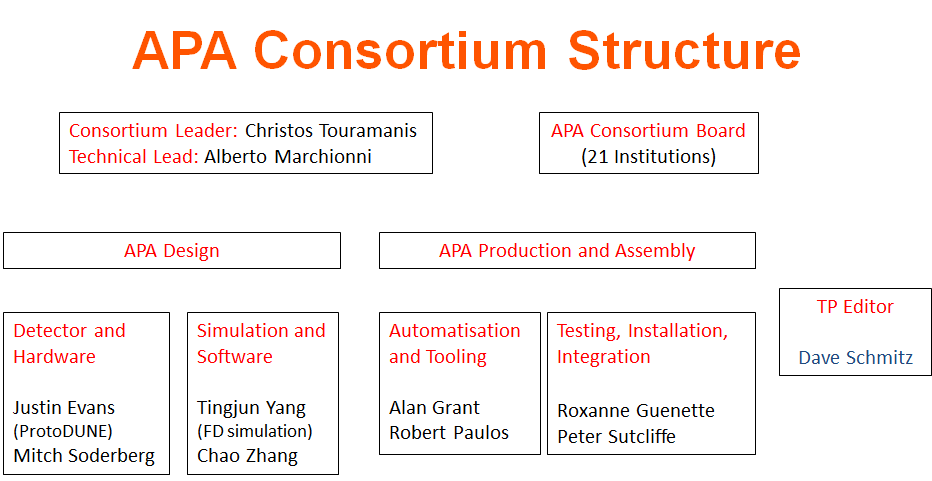
\includegraphics[width=0.95\textwidth,trim=0mm 0mm 0mm 0mm,clip]{apa-consortium-structure.png}
\end{dunefigure}


%%%%%%%%%%%%%%%%%%%%%%%%%%%%%%%%%%%%%%
\subsection{Planning Assumptions}
\label{sec:fdsp-apa-org-assmp}

The planning assumptions are based on having 8-9 APA assembly lines, at different locations in the UK and the US. 
We assume about one year of setup time for the factories.
It will take of the order 50 shifts to construct a single APA. Assuming a multi-shift system, we will be able to construct the 150 APAs required for one \SI{10}{kton} module within about two years.

%%%%%%%%%%%%%%%%%%%%%%%%%%%%%%%%%%%%%%
\subsection{WBS and Responsibilities}
\label{sec:fdsp-apa-org-wbs}

Here, we only discuss the top-level WBS elements, which are i)~design, engineering and R\&D, ii)~production setup, iii)~production, iv)~integration, and v)~installation.

The validation of the design is mainly a responsibility of the university groups and BNL, while engineering and the production setup will be developed at PSL in Madison (US) and Daresbury Laboratory (UK), where the APAs for ProtoDUNE have been built, with contributions from university groups. In addition to PSL and Daresbury Laboratory, the University of Chicago and Yale University have been identified as candidate sites for the production. The production sites will require significant contributions from university groups during the production process. 

In total, we expect half of the APAs to be produced in the US and half in the UK. The steel for the frames is most likely to be bought from a single vendor. The assembly of the frames will be performed in the US and the UK separately. The options to assemble the frames in house or in collaboration with industrial partners are still being explored. 

Another large component are the various types of boards. Design modifications relative to ProtoDUNE are the responsibility of BNL. The boards will be produced by industry, while the testing will be distributed among Consortium institutions. The shipping of the APAs is the responsibility of the production factories in the US and the UK.  The integration and installation are a joint responsibility of the Consortium, with ANL providing the interface with the technical coordination group.


%%%%%%%%%%%%%%%%%%%%%%%%%%%%%%%%%%%%%%%
\subsection{High-level Milestones and Schedule}
\label{sec:fdsp-apa-org-cs}

The high-level milestones for the period 2018 to 2024 are given in Table~\ref{tab:milestones} for the periods before and after the TDR. The final design of the APAs to be proposed in the TDR will be informed by the experience of the ProtoDUNE APA production and performance, which will be reviewed in early 2019. Additional design considerations that cannot be directly tested through ProtoDUNE, such as the two-APA assembly and the related cabling issues, will require a full test with cabling of a two-APA assembly also in early 2019. The production schedule, the required number of assembly lines, and the location of the production factories will depend on the improvements of the wire winding procedures, which will formally be reviewed in January 2019. The post-TDR milestones are driven by the high-level international project milestones and are based on a schedule with one year factory preparation and about two years of APA construction time.

\begin{dunetable}[APA design and construction milestones]{ll}{tab:milestones}{APA design and construction milestones}
Date &  Milestone   \\ \toprowrule
\multicolumn{2}{c}{Pre-TDR}\\
 December 2018 & Test 2-APA assembly   \\
 January 2019 & Formal review of complete modifications to the winder design\\
 February 2019 & Formal review of ProtoDUNE APA performance \\
February 2019 & Complete assembly test of FD prototype APA\\
March 2019 & Decision on location of factories and required number of assembly lines \\
March 2019 & APA cost estimate for Far Detector \SI{10}{kton} module \\
March 2019 & APA schedule for Far Detector \SI{10}{kton} Module \\
April 2019 & APA section of Technical Design Report delivered \\
\multicolumn{2}{c}{Post-TDR}\\
2020 & Preparation of APA factories \\
2021 -- 2023 & Construction of APAs \\
2022/3 & Installation of APAs in Far Detector 1\\
2024 & Commissioning of Far Detector 1 \\
\end{dunetable}